\documentclass[a4paper,14pt]{extarticle}

\usepackage[utf8x]{inputenc}
\usepackage[T1,T2A]{fontenc}
\usepackage[russian]{babel}
\usepackage{hyperref}
\usepackage{indentfirst}
\usepackage{here}
\usepackage{array}
\usepackage{graphicx}
\usepackage{caption}
\usepackage{subcaption}
\usepackage{chngcntr}
\usepackage{amsmath}
\usepackage{amssymb}
\usepackage{pgfplots}
\usepackage{pgfplotstable}
\usepackage[left=2cm,right=2cm,top=2cm,bottom=2cm,bindingoffset=0cm]{geometry}
\usepackage{multicol}

\renewcommand{\le}{\ensuremath{\leqslant}}
\renewcommand{\leq}{\ensuremath{\leqslant}}
\renewcommand{\ge}{\ensuremath{\geqslant}}
\renewcommand{\geq}{\ensuremath{\geqslant}}
\renewcommand{\epsilon}{\ensuremath{\varepsilon}}
\renewcommand{\phi}{\ensuremath{\varphi}}

\counterwithin{figure}{section}
\counterwithin{equation}{section}
\counterwithin{table}{section}
\newcommand{\sign}[1][5cm]{\makebox[#1]{\hrulefill}} % Поля подписи и даты
\graphicspath{{pics/}} % Путь до папки с картинками
\captionsetup{justification=centering,margin=1cm}
\def\arraystretch{1.3}

\usepackage{courier}

\usepackage{listings}
\lstset{ %
extendedchars=\true,
keepspaces=true,
language=C,						% choose the language of the code
basicstyle=\footnotesize,		% the size of the fonts that are used for the code
numbers=left,					% where to put the line-numbers
numberstyle=\footnotesize,		% the size of the fonts that are used for the line-numbers
stepnumber=1,					% the step between two line-numbers. If it is 1 each line will be numbered
numbersep=5pt,					% how far the line-numbers are from the code
backgroundcolor=\color{white},	% choose the background color. You must add \usepackage{color}
showspaces=false				% show spaces adding particular underscores
showstringspaces=false,			% underline spaces within strings
showtabs=false,					% show tabs within strings adding particular underscores
frame=single,           		% adds a frame around the code
tabsize=2,						% sets default tabsize to 2 spaces
captionpos=b,					% sets the caption-position to bottom
breaklines=true,				% sets automatic line breaking
breakatwhitespace=false,		% sets if automatic breaks should only happen at whitespace
escapeinside={\%*}{*)},			% if you want to add a comment within your code
postbreak=\raisebox{0ex}[0ex][0ex]{\ensuremath{\color{red}\hookrightarrow\space}},
texcl=true,
}

\lstset{basicstyle=\footnotesize\ttfamily,breaklines=true}

\begin{document}

\begin{titlepage}
\begin{center}
	\textbf{Санкт-Петербургский Политехнический Университет \\Петра Великого}\\[0.3cm]
	\small Институт компьютерных наук и технологий \\[0.3cm]
	\small Кафедра компьютерных систем и программных технологий\\[4cm]
	
	\textbf{ОТЧЕТ}\\ \textbf{о лабораторной работе}\\[0.5cm]
	\textbf{<<Использование стандартных подпрограмм для приближенного\\ вычисления интеграла>>}\\[0.1cm]
	\textbf{Вычислительная математика}\\[8.0cm]
\end{center}

\begin{flushright}
	\begin{minipage}{0.48\textwidth}
		\begin{flushleft}
			\small \textbf{Работу выполнил студент}\\[3mm]
			\small группа 23501/4 \hspace*{6mm} Дьячков В.В.\\[5mm]
			
			\small \textbf{Преподаватель}\\[5mm]
		 	\small \sign[3cm] \hspace*{5mm} к.т.н., доц. Цыган В.Н.\\[0.5cm]
		\end{flushleft}
	\end{minipage}
\end{flushright}

\vfill

\begin{center}
	\small Санкт-Петербург\\
	\small \the\year
\end{center}
\end{titlepage}

\section{Техническое задание}

\textbf{Вариант 5:} Составить процедуру вычисления нормы матрицы $R = A\cdot A^{-1} - E$, где норма матрицы $R$ равна:
\[
\norm{R} = \max_k \sum_j |R_{kj}|.
\]

Используя подпрограммы \textbf{DECOMP} и \textbf{SOLVE}, вычислить $A^{-1}$ по заданной матрице $A$. Для различных значений $p$ вычислить нормы матриц $R$.

\section{Исходные данные}

Исходная матрица $A$:
\[
\begin{pmatrix}
  p+13 & 2  & 8  & -7 & 7  & 5  & -7 & -7 \\
  7    & 2  & -4 & 2  & 3  & 3  & -1 & -2 \\
  -7   & 2  & 1  & 3  & 6  & -6 & -3 & -4 \\
  -2   & -8 & -6 & -1 & 6  & 2  & 1  & -4 \\
  0    & 4  & -7 & 1  & 22 & 0  & -6 & -6 \\
  0    & -3 & -6 & 6  & 4  & 13 & 0  & 6  \\
  -8   & -6 & -4 & 7  & -5 & -5 & -2 & 1  \\
  5    & 5  & -2 & -2 & -3 & 0  & -7 & 14
\end{pmatrix}
\]

Значения параметра $p$:
\begin{multicols}{5} 
	$p = 1$ \\
	$p = 0.1$ \\
	$p = 0.01$ \\
	$p = 0.001$ \\
	$p = 0.00001$
\end{multicols}

\section{Выполнение работы}

В процессе работы была разработана программа на языке \textbf{C++}, вычисляющая искомую матрицу $R$ (см.~листинг~\ref{code:main}). Для упрощения взаимодействия с матрицами был разработан класс \textbf{Matrix} (см.~листинг~\ref{code:matrix}). Для нахождения обратной матрицы использовались подпрограммы \textbf{DECOMP} и \textbf{SOLVE}. На рисунках \ref{fig:p1} -- \ref{fig:p5} изображен вывод программы для заданных значений параметра $p$.

\begin{figure}[H]
\begin{center}
	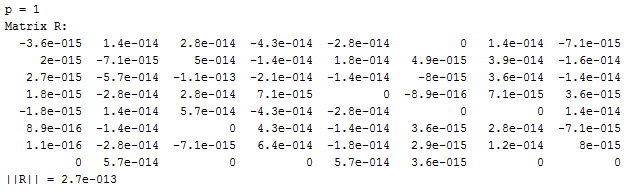
\includegraphics[scale=0.88]{1}
	\caption{Вывод программы при $p = 1$}
	\label{fig:p1}
\end{center}
\end{figure}

\vspace{-1.3cm}

\begin{figure}[H]
\begin{center}
	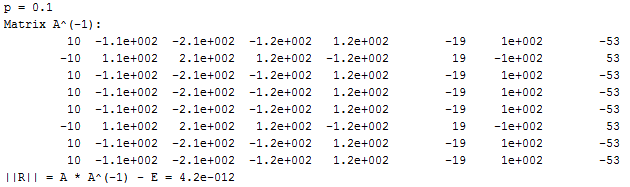
\includegraphics[scale=0.88]{2}
	\caption{Вывод программы при $p = 0.1$}
	\label{fig:p2}
\end{center}
\end{figure}

\vspace{-1cm}

\begin{figure}[H]
\begin{center}
	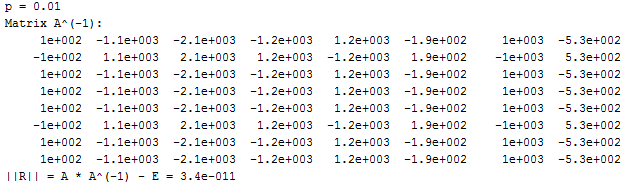
\includegraphics[scale=0.88]{3}
	\caption{Вывод программы при $p = 0.01$}
	\label{fig:p3}
\end{center}
\end{figure}

\vspace{-1cm}

\begin{figure}[H]
\begin{center}
	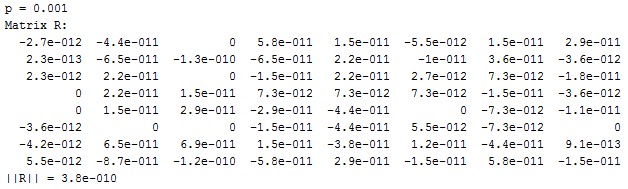
\includegraphics[scale=0.88]{4}
	\caption{Вывод программы при $p = 0.001$}
	\label{fig:p4}
\end{center}
\end{figure}

\vspace{-1cm}

\begin{figure}[H]
\begin{center}
	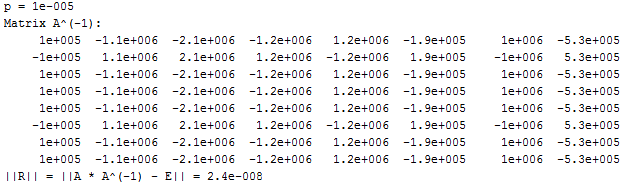
\includegraphics[scale=0.88]{5}
	\caption{Вывод программы при $p = 0.00001$}
	\label{fig:p5}
\end{center}
\end{figure}

\newpage

\section{Результаты}

Сравним значения, получившиеся путем изменения параметра p:

\begin{table}[H]
\begin{center}
	\caption{Полученные результаты}
	\def\tabcolsep{15pt}
	\begin{tabular}{|c|c|c|c|c|c|}
		\hline
		$p$ &
		$1$ &
		$0.1$ &
		$0.01$ &
		$0.001$ &
		$0.00001$ \\
		\hline
		$||R||$ &
		$2.7\cdot 10^{-13}$ &
		$4.2\cdot 10^{-12}$ &
		$3.4\cdot 10^{-11}$ &
		$3.8\cdot 10^{-10}$ &
		$2.4\cdot 10^{-8}$ \\
	    \hline	
	\end{tabular}
	\label{tab:results}
\end{center}
\end{table}

Из таблицы \ref{tab:results} видно, что при уменьшении параметра $p$ значения элементов матрицы $R$ увеличиваются, и, следовательно, ее норма растет. Выясним, сохраняется ли тенденция при еще меньших значениях параметра $p$. Для этого будем изменить $p$ в диапазоне $10^{-14}~\div~1$. Полученный график изменения нормы матрицы $R$ в зависимости от параметра $p$ в логарифмической шкале изображен на рисунке \ref{fig:p}. Из графика видно, что значение $||R||$ практически линейно зависит от параметра $p$.

\begin{figure}[H]
\begin{center}
	\begin{tikzpicture} [every plot/.append style={thick}]
		\begin{axis}[
			height=0.4\textheight,
			width=0.9\textwidth,
			legend pos=north east,
			xlabel={$\lg p$},
			ylabel={$\lg ||R||$},
			xlabel near ticks,
			ylabel near ticks,
			xmode=log,
			log basis x=10,
			xmin=1e-16,
			xmax=1e2,
			xtick={1e-14, 1e-12, 1e-10, 1e-8, 1e-6, 1e-4, 1e-2, 1e0},
			ymode=log,
			log basis y=10,
			ymin=1e-16,
			ymax=1e4,
			grid=major
		]
		\addplot table[x=p,y=norm_r,col sep=comma]{data/p.csv};
		\end{axis}
	\end{tikzpicture}
	\caption{Зависимость $||R||$ от $p$ в логарифмической шкале}
	\label{fig:p}
\end{center}
\end{figure}



\section{Выводы}

Таким образом можно сделать вывод, что даже при очень небольшом измениии матрицы $A$, значения обратной матрицы $A^{-1}$ увеличиваются на порядок, что ведет к снижению точности и увеличению значений матрицы $R = A\cdot A^{-1} - E$ и ее нормы.

\newpage

\section*{Приложение}

\captionof{lstlisting}{main.cpp}
\lstinputlisting[
	basicstyle=\scriptsize,	
	numberstyle=\scriptsize,
	label=code:main
]{main.cpp}
\parindent=1cm

\captionof{lstlisting}{matrix.h}
\lstinputlisting[
	basicstyle=\scriptsize,	
	numberstyle=\scriptsize,
	label=code:matrix
]{matrix.h}
\parindent=1cm

\end{document}
